\documentclass[12pt]{article}
\usepackage[utf8]{inputenc}
\usepackage {mathtools, graphicx, amsfonts, amssymb, comment}
\usepackage{enumerate}
\usepackage{geometry}
\usepackage{subcaption}
\usepackage{float}
\usepackage[backend=bibtex,sorting=ynt]{biblatex}
\usepackage{hyperref}

\addbibresource{bibliography.bib}
\geometry{margin=1.25in}

% http://tex.stackexchange.com/questions/65849/confusion-onehalfspacing-vs-spacing-vs-word-vs-the-world
\linespread{1.25}

\title{Math 414 Final Project}
\author{Matt Gaikema \\ Will Argueta}
\date{April 2016}

\begin{document}

\maketitle

%%%%%%%%%%%%%%%%
% INTRODUCTION %
%%%%%%%%%%%%%%%%
\section{Introduction}

In order to efficiently send and receive images, it is often useful to compress them, 
since much of the data may be irrelevant or redundant.
Also, since plaintext consumes less memory than image files, it becomes important to encode images,
or store them as plaintext.
One of the many ways of accomplishing this is through wavelets.

There are two types of image compression: lossy and lossless.
\textbf{Lossless} compression means that every bit of information is recovered from the compressed data,
while \textbf{lossy} compression occurs when redundant information is eliminated.
The GIF is an example of lossless compression, while the JPEG is lossy.

The JPEG 2000 is one method of image compression which uses wavelets.
It was created in 2000 by the Joint Photographic Experts Group with the aim of replacing the original JPEG standard, 
which uses the Discrete Cosine Transform and was created in 1992.
The file extension is \verb|.jp2|, compared with the typical JPEG extension of \verb|.jpg|.

% http://www.verypdf.com/pdfinfoeditor/jpeg-jpeg-2000-comparison.htm
\begin{figure}[h]
	\centering
	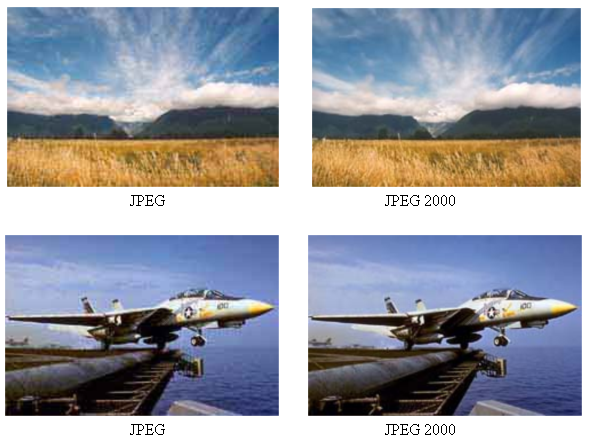
\includegraphics[scale=0.4]{resources/comparison.png}
	\caption{Two images compressed using JPEG and JPEG 2000.\cite{comparison}}
	\label{fig:compare}
\end{figure}

There are a few advantages of the JPEG 2000 over the JPEG,
thanks to the JPEG 2000's use of wavelets.
First, JPEG 2000 can be lossy or lossless, while JPEG compression is always lossy.
This means that JPEG 2000 produces images of much higher quality.
Figure \ref{fig:compare} shows two images compressed both using JPEG and JPEG 2000.

Of course, despite the advantages of the JPEG 2000, it is rarely used today, 
while the JPEG is still very popular.
The main reason is computation.\cite{alternative} 
Adopting the JPEG 2000 would have required rewriting much software, 
since it was not backwards-compatable with the JPEG.
Many companies were unwilling to add support for it since it wasn't popular,
and many consumers didn't use it since there was little support for it,
creating an unfortunate cycle. 
Additionally, the JPEG 2000 requires more computing power, which was not as abundant in 2000 as it is today.
To this day, few websites and no major web browsers support it.


%%%%%%%%%%%%%%%%%%%%%%%%%%%
% MATHEMATICAL BACKGROUND %
%%%%%%%%%%%%%%%%%%%%%%%%%%%
\section{Mathematical Background}
% https://en.wikipedia.org/wiki/JPEG_2000

The JPEG 2000's use of the Discrete Wavelet Transform is what makes it superior to the JPEG.\cite{how}
The Discrete Cosine Transform (DCT), which is used by the JPEG, compresses the image into 8x8 blocks
and places them consecutively in the file.
The blocks are compressed individually.
This is the reason for "blockiness" in compressed JPEG images.

Wavelet compression converts the image into a series of wavelets, which can be more easily stored than pixel blocks.

The JPEG 2000 compression algorithm consists of four basic steps: 
preprocess, transformation, quantization, and encoding\cite{whydomath}.

% A lossy transform on the baby picture.
\begin{figure}[h]
	\centering
	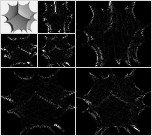
\includegraphics[scale=0.6]{resources/lossybaby.png}
	\caption{DWT using the lossy 9/7 filter.}
	\label{fig:lossybaby}
\end{figure}

% A lossless transform on the baby picture.
\begin{figure}[h]
	\centering
	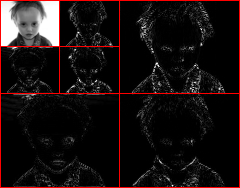
\includegraphics[scale=0.6]{resources/losslessbaby.png}
	\caption{DWT using the lossless 5/3 filter.}
	\label{fig:losslessbaby}
\end{figure}

\begin{enumerate}
	
	\item\textbf{Preprocecessing:}
	If the image is a color image, the image needs to be converted to the YCbCr color space\cite{colorspace}
	from the standard RGB color space.

	After the color space transform, sometimes the image will be split up into different tiles of equal size,
	but this is optional.
	
	\item\textbf{Transform:}
	The Discrete Wavelet Transform is the most impportant feature of the JPEG 2000.
	In the case of a lossy compression, a Cohen-Daubechies-Feauveau (CDF) 9/7 wavelet is used,
	while the CDF 5/3 wavelet is used for lossless compression.
	In both cases, between two and three iterations are computed.
	
	\item\textbf{Quantization:}
	Quantization refers to the process of compressing a range of values into a single value,
	and is used in lossy compression.
	If the compression is lossless, then no quantization is done.
	Figure \ref{fig:losslessbaby} is encoded and the algorithm is completed.
	
	In a lossy compression, more work must be done.
	The quantization scheme used is not unlike that used by JPEG on the 8x8 blocks,
	where two iterations of the DWT results in seven blocks.
	A floor function is applied to each of the wavelet coefficients.
	
	\item\textbf{Encoding:}
	For encoding, Embedded Block Coding with Optimized Truncation, or EBCOT, is used.
	
\end{enumerate}

\begin{figure}[h]
	\centering
	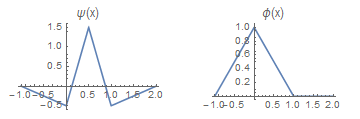
\includegraphics[scale=0.9]{resources/lossless_family.png}
	\caption{Wavelet and scaling functions for the CDF 5/3 transform.}
	\label{fig:lossless_family}
\end{figure}

\begin{figure}[h]
	\centering
	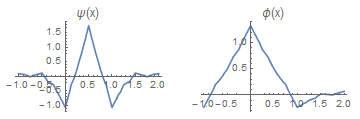
\includegraphics[scale=0.9]{resources/lossy_family.png}
	\caption{Wavelet and scaling functions for the CDF 9/7 transform.}
	\label{fig:lossy_family}
\end{figure}

\subsection{The CDF Wavelet}
% http://www.ams.org/samplings/feature-column/fcarc-image-compression

The CDF Wavelet is a biorthogonal wavelet, which satisfies four properties\cite{old}:
\begin{itemize}
	\item The scaling function, $\phi(x)$, is always symmetric.
	\item The wavelet function, $\psi(x)$, is always symmetric or anti-symmetric.
	\item The wavelet filters are finite.
	\item The coefficients of the wavelet filters have the form $\frac{z}{2^n}$, with $z\in\mathbb{Z}$ and $n\in\mathbb{N}$.
\end{itemize}

%\bigskip
%\noindent
%The wavelet transform on an image produces as many coefficients as there are pixels.


%%%%%%%%%%%%%%%
% APPLICATION %
%%%%%%%%%%%%%%%
\section{Application}

The source code for the implemented transformations can be found at \cite{repo},
in the file \href{https://raw.githubusercontent.com/TexAgg/Math-414-Final-Project/master/main.wl}{main.wl}.


%%%%%%%%%%%%%%
% CONCLUSION %
%%%%%%%%%%%%%%
\section{Conclusion}

The JPEG 2000 could easily be the next standard for image compression, if only people would use it.


%%%%%%%%%%%%%%
% REFERENCES %
%%%%%%%%%%%%%%
\printbibliography[]


\end{document}
